\documentclass[12pt,twoside]{article}

% *** Set page dimensions ***
\raggedbottom
\parindent=0in
%\setlength{\topmargin}{-0.5in}
%\setlength{\oddsidemargin}{0.1875in}
%\setlength{\evensidemargin}{0in}
%\setlength{\textheight}{8.5in}
%\setlength{\textwidth}{6.225in}
%\addtolength{\oddsidemargin}{-0.7in}
%\addtolength{\evensidemargin}{-1.2in}
%\setlength{\oddsidemargin}{-0.2in}
%\setlength{\evensidemargin}{-0.2in}
%\addtolength{\textwidth}{1.4in}
%\addtolength{\topmargin}{-.875in}
%\addtolength{\textheight}{2.00in}

% *** Packages ***
\usepackage{alltt}
\usepackage{tocloft}
\usepackage{graphicx}
\usepackage{lscape}
\usepackage{amssymb}
\usepackage{float}
\usepackage{amsmath}
\usepackage{gensymb}
%\usepackage{subfigure}
\usepackage{lscape}
\usepackage{epsfig}
\usepackage{enumerate}
\usepackage{multicol}
\usepackage{fancyhdr}
\usepackage{epstopdf}
\usepackage{hyperref}
\usepackage{listings}

% *** Table of contents and Sectioning *** 
\setcounter{secnumdepth}{0}
\setcounter{tocdepth}{5}

% *** Table of contents and Sectioning *** 
\newcommand{\next}{\addtocounter{enumi}{9} \item}
\newcommand{\now}[1]{\setcounter{enumi}{#1}}
\newcommand{\Z}{\mbox{\sf Z\hspace{-1.5mm}Z}}
\newcommand{\R}{\mbox{\rm I\hspace{-0.75mm}R}}
\columnsep=0.75in

% *** Shortcuts for syntax ***
\newcommand{\ds}{\displaystyle }
\newcommand{\vsc}{\vspace{4mm}}
\newcommand{\dd}[1]{\frac{d}{d{#1}} \,} 
\newcommand{\ddx}{\frac{d}{dx} \,} 
\newcommand{\ddy}{\frac{d}{dy} \,} 
\newcommand{\ddz}{\frac{d}{dz} \,} 
\newcommand{\dydx}{\frac{dy}{dx} \,} 
\newcommand{\dydt}{\frac{dy}{dt} \,} 
\newcommand{\dfdx}{\frac{df}{dx} \,} 
\newcommand{\ddt}[1]{  \frac{d{#1}}{dt} }
\newcommand{\pp}[2]{  \frac{\partial{#1}}{\partial {#2}} }
\newcommand{\zx}{\frac{\partial z}{\partial x} \,}
\newcommand{\zy}{\frac{\partial z}{\partial y} \,}
\newcommand{\limh}{\lim_{h \rightarrow 0} \;}
\newcommand{\diff}{\frac{d}{dx} \,}
\newcommand{\de}{\Delta}
\renewcommand{\thesection}{\Roman{section}}
\newcommand{\bfr}{\begin{flushright}}
\newcommand{\efr}{\end{flushright}}
\newcommand{\dx}{\frac{\partial f}{\partial x} \,}
\newcommand{\dy}{\frac{\partial f}{\partial y} \,}
\newcommand{\p}{\partial}
\newcommand{\vi}{\vec{i}}
\newcommand{\vj}{\vec{j}}
\newcommand{\vk}{\vec{k}}
\newcommand{\lan}{\left\langle}
\newcommand{\ran}{\right\rangle}
\newcommand{\reading}[1] { {\em Reading: #1}}
\renewcommand{\Pr}{ \mbox{Pr}}

% *** Commands related to textbook references
\newcommand{\problem}{{\bf Problem.} }

% *** Footnoting with symbols ***
\long\def\symbolfootnote[#1]#2{\begingroup%
\def\thefootnote{\fnsymbol{footnote}}\footnote[#1]{#2}\endgroup}

% *** Defining a boxed note ***
\floatstyle{boxed}
\newfloat{noteinbox}{htb}{loa}
\newenvironment{boxnote}{\begin{noteinbox}[H]}{\end{noteinbox}}

\newcommand{\Question}{ {\bf Question: }  }
\newcommand{\Example}[1]{ {\bf Example: } {\em #1} }
\newcommand{\ExampleCont}[1]{ {\em #1} }

% *** Define the boxed Week #/summary at the beginning/end of every chapter ***
\newcommand{\sectionbox}[1]{% 
\begin{tabular}{|p{6in}|}%
\hline%
\ \\ %
{\Large {\bf {#1}}}  \\%
\ \\%
\hline%
\end{tabular}}

% *** Shortcuts *** 
\newcommand\goals{\large {\bf {Goals:}}}
\newcommand\setfont{ }

% *** Week commands: overwritten in each notes file
\newcommand{\Week}{Null-InPreambleCommon}
\newcommand{\WeekTitle}{Null-InPreambleCommon}
\newcommand{\Course}{MNTC P04}
\newcommand{\SetNum}{1 }
\newcommand{\topic}[1]{
\newpage
\setcounter{page}{1}
\fancyhead[LE,RO]{#1 - \thepage}
}

% *** Setup Latex for the large version of the files ***
%\usepackage[landscape]{geometry}
\usepackage[letterpaper,landscape,hmargin={.8in,.8in},vmargin={1in,0.2in}]{geometry}

% Remove paragraph indents
\setlength{\parindent}{0pt}

% Spacing at the top for the header is too large by default
\setlength{\voffset}{-5ex}

% **** RENEW SCALING COMMANDS HERE ****
% *** Text in boxes ***
\renewenvironment{boxnote}{\begin{noteinbox}[H] \huge}{\end{noteinbox}} 

% *** Chapter lead in/summary boxes ***
\renewcommand{\sectionbox}[1]{% 
\begin{tabular}{|p{9.5in}|}%
\hline%
\ \\ %
{\huge {\bf {#1}}}  \\%
\ \\%
\hline%
\end{tabular}}

% *** 'Section'' commands, which are sometimes used for spacing
% From http://zoonek.free.fr/LaTeX/LaTeX_samples_section/0.html
\makeatletter
 \renewcommand\section{\@startsection {section}{1}{\z@}%
                                    {-3.5ex \@plus -1ex \@minus -.2ex}%
                                    {0.3ex \@plus.2ex}%
                                    {\setfont\bf}}

 \renewcommand\subsection{\@startsection {subsection}{1}{\z@}%
                                    {-3.5ex \@plus -1ex \@minus -.2ex}%
                                    {0.3ex \@plus.2ex}%
                                    {\setfont\bf}}

% *** 'Goals' should be larger in the overheads ***
\renewcommand\goals{\huge {\bf {Goals:}}}
\renewcommand\setfont{\huge }

\thispagestyle{empty}

\setfont 

\newcommand{\WeekTitleOne}{Derivatives - Foundations}
\newcommand{\WeekTitleTwo}{Derivatives - Linearization and Applications}
\newcommand{\WeekTitleThree}{Derivatives - Modeling}
\newcommand{\WeekTitleFour}{Integrals - Foundations}
\newcommand{\WeekTitleFive}{Integrals - Techniques}
\newcommand{\WeekTitleSix}{Integrals - Modeling}
\newcommand{\WeekTitleSeven}{Differential Equations - }
\newcommand{\WeekTitleEight}{Differential Equations - }
\newcommand{\WeekTitleNine}{Differential Equations - }
\newcommand{\WeekTitleTen}{Linear Algebra - }
\newcommand{\WeekTitleEleven}{Linear Algebra - }
\newcommand{\WeekTitleTwelve}{Linear Algebra - }



\begin{document}
\setfont
\pagestyle{fancy}
\renewcommand{\Week}{3 }
\renewcommand{\WeekTitle}{\WeekTitleThree }

\fancyhead[LE,RO]{Week \Week}  % default, usually only for first page
\fancyfoot{}
\sectionbox{Week \#\Week: \WeekTitle}


\vspace{5mm}
\goals
\begin{itemize}
\item Calculate and interpret the first and second derivatives, as
  well as higher order derivatives.
\item Define and calculate Taylor Polynomials.
\item Use MATLAB to graph and compare functions with their Taylor
  polynomial approximations.
\item Find and use critical points for global and local optimization
  problems.
\item Use MATLAB optimizers and equation solvers to identify optimal
  values and critical points.
\end{itemize}

\vspace{5mm}


\newpage
\topic{Second and Higher Derivatives}
\subsection*{Second and Higher Derivatives}


The information about the graph of a function $f$ provided by the sign
of $f'(x)$ and $f''(x)$ on an interval $(a,b)$ is expressed in the
following table. ($a$ and $b$ are assumed to be finite.)

{\huge
\vsc
\begin{center}
\begin{tabular}{|l|l|} \hline
\qquad \qquad \qquad \qquad \qquad  \qquad \qquad & \qquad  \qquad \qquad \qquad \qquad  \qquad \qquad \\
\qquad $f'(x) > 0 {\mbox{ on }} (a,b)$  &  \qquad $f$ increasing on $[a,b]$  \\
\qquad \qquad \qquad \qquad \qquad & \qquad \qquad \qquad  \qquad \qquad \\
 \hline
\qquad \qquad \qquad \qquad \qquad & \qquad \qquad \qquad  \qquad \qquad \\
\qquad $f'(x) < 0 {\mbox{ on }} (a,b)$  &  \qquad $f$ decreasing on $[a,b]$  \\
\qquad \qquad \qquad \qquad \qquad & \qquad \qquad \qquad  \qquad \qquad \\
 \hline
\qquad \qquad \qquad \qquad \qquad & \qquad \qquad \qquad  \qquad \qquad \\
\qquad $f''(x) > 0 {\mbox{ on }} (a,b)$  &  \qquad $f$ concave up on $[a,b]$  \\ \qquad \qquad \qquad \qquad \qquad & \qquad \qquad \qquad  \qquad \qquad \\
\hline
\qquad \qquad \qquad \qquad \qquad & \qquad \qquad \qquad  \qquad \qquad \\
\qquad $f''(x) < 0 {\mbox{ on }} (a,b)$  &  \qquad $f$ concave down on $[a,b]$ \qquad  \qquad  \\ 
\qquad \qquad \qquad \qquad \qquad & \qquad \qquad \qquad  \qquad \qquad \\
\hline
\end{tabular}
\end{center}
}
\setfont

\newpage

Aside from their graphical interpretation, second derivatives
frequently have important physical interpretations in kinematics
problems.

\problem If $x(t) = 4 \sin(2t)$ gives the position of a particle at
time $t$, what is particle's {\bf speed} at $\ds t=\frac{\pi}{6}$?

\vfill

For the same particle, what is its {\bf acceleration} at
$\ds t=\frac{\pi}{6}$?

\vfill

\newpage



While their interpretations are not as immediately obvious, it is
possible to compute 3rd and higher derivatives of function if we want.

\problem Find the first four derivatives of the function
$$f(x) = 7 (2^x) + \ln(x).$$


\newpage
\topic{Taylor Polynomials}
\subsection*{Taylor Polynomials}

One application of higher derivative information is to help us build
{\bf polynomial approximations} to complicated functions.

Previously we found a formula for linear approximations to functions
$f(x)$ around a point $x=a$:

\vspace{1.5in}

This linear approximation, or tangent line formula, can also be called
the {\bf Taylor polynomial of degree 1 approximating $f(x)$ near
  $x=a$.}

\newpage

Sketch the graph of $\cos(x)$ around $x=0$, and add its
  tangent line based at $x=0$.


\includegraphics[width=3in]{graphics/empty_graph_square_12}


The linearization or tangent line is clearly a very
  limited approximation to this function.  What might be a {\em
    slightly} more complex form of function that would work better in
  this case?

\vfill

\newpage

\begin{boxnote}

{\bf Taylor Polynomial of Degree 2}
\vspace{1in}

$$ f(x) \approx ~~~~~f(a) ~~~~~+ f'(a) (x-a) ~~~~~+ \frac{f''(a)}{2} (x-a)^2$$  

\vspace{1in}

is a {\em quadratic} approximation to $f(x)$ near $x=a$.
\end{boxnote}


For values of $x$ close to $a$ do you think this
  quadratic approximation will be a better or worse approximation than
  the tangent line?  Why?

\vfill

\newpage
\topic{Taylor Polynomials - Examples}

\problem Find the quadratic Taylor approximation to \\$f(x) = \cos(x)$
  near $x=0$.

\vfill

\newpage

\problem Use MATLAB to draw the graph of $\cos(x)$ around $x=0$, and
add both its 1st and 2nd degree Taylor polynomial approximations for
$x$ near 0.


\newpage

There is a very good reason for the particular form of the Taylor
polynomial.

\problem What mathematical features will $f(x)$ and its 2nd degree
Taylor approximation share at $x=a$?

\vfill

\newpage
\topic{Taylor Polynomials of Higher Degree}
\subsection{Taylor Polynomials of Higher Degree}

\problem If we wanted a still-better approximation for a function
$f(x)$ near a specific point $x=a$, how could we generalize our
earlier 1st and 2nd degree Taylor polynomials?

\vfill

\newpage 

This is the general formula for the terms in a Taylor polynomial, up
to degree $n$.  \\ 

$$ f(x) \approx ~~f(a) ~~+ f'(a) (x-a) ~~+ \frac{f''(a)}{2} (x-a)^2 + \ldots 
+ \frac{f^{(n)}(a)}{n!} (x-a)^n$$   \\

\begin{itemize}
\item $f^{(n)}$ means ``the $n$-th derivative of $f$''. \\
\item $n!$ means ``$n$ factorial''
\end{itemize}

\newpage
\subsection*{Higher Degree Taylor Polynomials - Example}

Consider the function $f(x) = \sin(x)$.

\problem Find the first four derivatives of $f(x)$.

\newpage

\problem Write out the Taylor poylnomial of degree 5 for
$f(x) = \sin(x)$.

\vfill

\problem Write out the general form of the Taylor poylnomial of degree
$n$ for $f(x) = \sin(x)$.

\vfill

\newpage

\problem Use MATLAB to plot the graph of $f(x) = \sin(x)$ and the
Taylor polynomial approximations up to degree 5.

\newpage

MATLAB Demo of increasing higher degrees.


\newpage
\topic{Critical Points}

\section*{Critical Points} 

\begin{boxnote}

  If $f(x)$ is defined on the interval $(a,b)$, then we call a point
  $c$ in the interval a {\bf critical point} if:
\begin{itemize}
	\item $f'(c) = 0$, or
	\item $f'(c)$ does not exist.
\end{itemize}
We will also refer to the point $(c,f(c))$ on the graph of $f(x)$ as a
critical point.  We call the function value $f(c)$ at a critical point
$c$ a {\bf critical value}.

\vsc
\end{boxnote}

\newpage

Technical Notes:
\begin{enumerate} 
\item By this definition, $f(c)$ must be {\bf defined} for
  $c$ to be a critical point.  

  Sketch $f(x) = 1/x$, and decide whether $x=0$ is a
    critical point.

\vfill
  Sketch $g(x) = |x|$, and decide whether $x=0$ is a
    critical point.

\vfill

\newpage

\item By the definition, if a function is defined on a closed
  interval, the endpoints of interval {\bf cannot} be critical points.

  Sketch the graph of $f(x) = \sqrt{x}$ and decide
    whether $x=0$ is a critical point.

\vfill

\newpage

Sketch the graph of $g(x) = \sqrt[3]{x}$ and decide
  whether $x=0$ is a critical point.

\vfill

\end{enumerate}

\newpage

\problem Identify all the critical points on the graph below, and
  characterize any other interesting points by continuity, limits, or
  other properties.

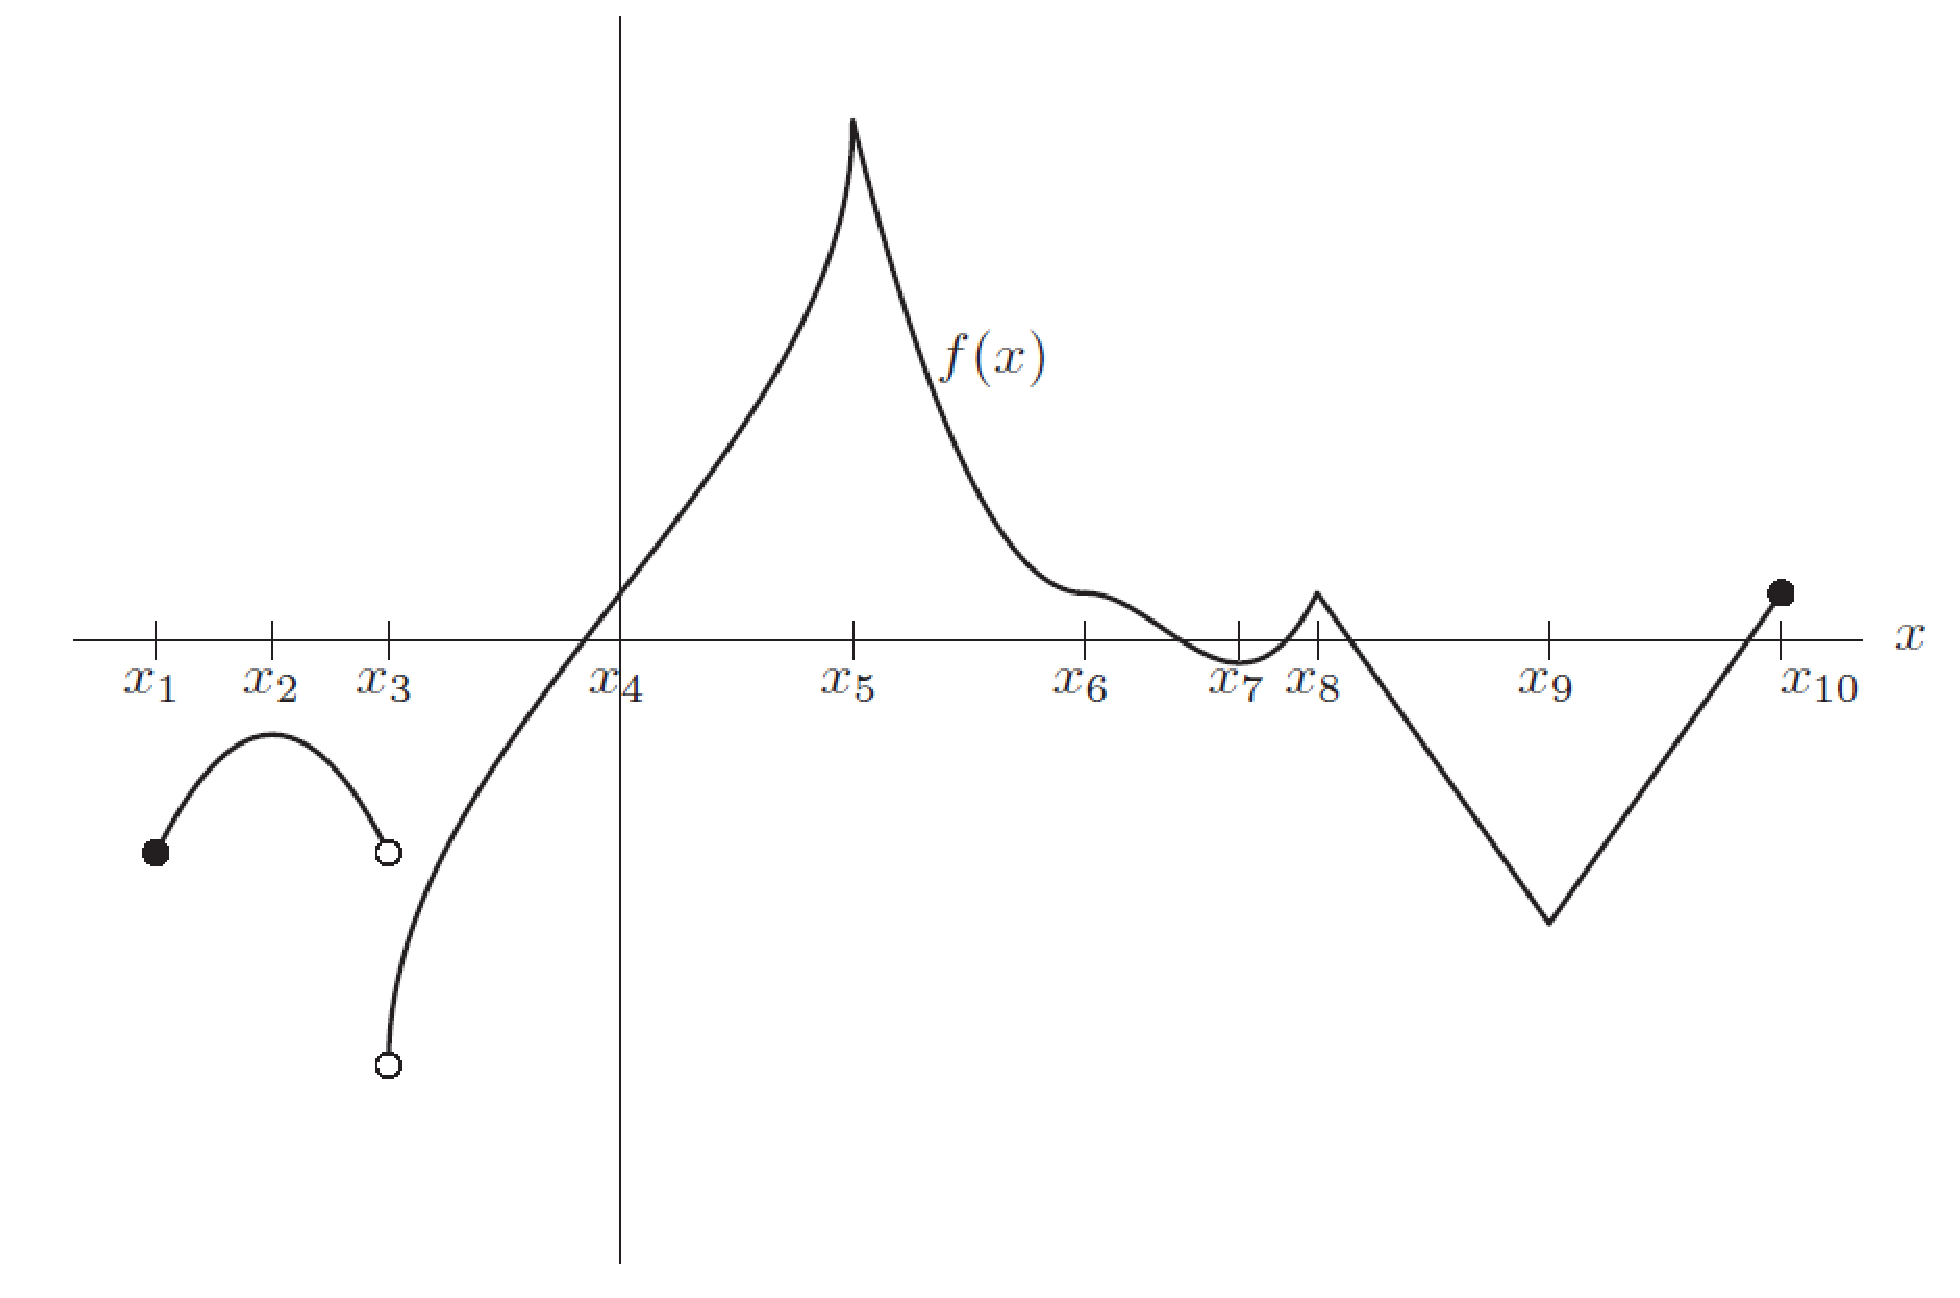
\includegraphics[width=8in]{graphics/notes06_crit_pnt_oddities}

\newpage

\topic{First and Second Derivative Sign Chart Example}

\problem Consider the function  
$$f(x) = \frac{x}{x^2 + 1}$$
Construct a sign chart for both $f'$ and $f''$, and use this information to
sketch $f(x)$.

\vfill
\newpage
\vfill

\hfill 
\includegraphics[width=4in]{graphics/empty_graph_square_12}

\newpage
\topic{Optimization - Introduction}
\subsection*{Optimization - Introduction}

\newpage
\topic{Optimization - Critical Points}
\subsection*{Optimization - Critical Points}




\end{document}

